\chapter{Modellazione dei Casi d'Uso}

\section{Attori e Casi d'Uso}

\begin{table}[!hbp]
	\centering
	\begin{tblr}{colspec=XX}
		\begin{minipage}[t]{\linewidth}
			\paragraph{Attori primari}
			\begin{itemize}
				\item UtenteRegistrato
				\item Cliente
				\item Farmacista
				\item Direttore
				\item Cliente non registrato
			\end{itemize}
		\end{minipage} &
		\begin{minipage}[t]{\linewidth}
			\paragraph{Attori secondari}
			\begin{itemize}
				\item Farmacista
			\end{itemize}
		\end{minipage} \\
	\end{tblr}
\end{table}

\begin{table}[!hbp]
	\centering
	\begin{tblr}{colspec=XX}
		\begin{minipage}[t]{\linewidth}
			\paragraph{Casi d'uso}
			\begin{enumerate}
				\item VisualizzaCatalogo % RF01, RF06
				\item AggiungiFarmaco % RF02
				\item CercaFarmaco % RF18
				\item ModificaFarmaco % RF03
				\item EliminaFarmaco % RF04
				\item RegistraCliente % RF05
				\item CreaOrdine % RF07, RF08, RF09, RF17
				\item GeneraOrdineAcquisto % RF10
				\item VisualizzaOrdiniAcquisto % RF11
				\item RegistraConsegnaOrdineAcquisto % RF12
				\item GeneraReport % RF13
				\item VisualizzaOrdiniFarmacia % RF14
				\item RitiraOrdine % RF15
				\item VisualizzaStoricoOrdini % RF16
				\item GeneraOrdineAcquistoFarmacista % RF19
			\end{enumerate}
		\end{minipage} &
		\begin{minipage}[t]{\linewidth}
			\paragraph{Casi d'uso di inclusione}
			\begin{enumerate}
				\item CercaFarmaco
				\item VisualizzaOrdiniFarmacia
				\item VisualizzaOrdiniAcquisto
			\end{enumerate}

			\paragraph{Casi d'uso di estensione}
			\begin{enumerate}
				\item GeneraOrdineAcquisto % RF10
			\end{enumerate}
		\end{minipage}
	\end{tblr}
\end{table}

\begin{table}[!ht]
	\centering
	\small
	\begin{tblr}{
		colspec = lllll,
		hlines,
		row{1} = {font=\bfseries}
	}
		Caso d'uso & Attori primari & {Attori \\ secondari} & Incl. / Ext. & Requisito \\
		VisualizzaCatalogo & UtenteRegistrato & -- & -- & {\Req{rf}{01} \\ \Req{rf}{06}} \\
		AggiungiFarmaco & Farmacista & -- & -- & \Req{rf}{02} \\
		ModificaFarmaco & Farmacista & -- & {Include \\ VisualizzaCatalogo} & \Req{rf}{03} \\
		EliminaFarmaco & Farmacista & -- & {Include \\ VisualizzaCatalogo} & \Req{rf}{04} \\
		RegistraCliente & {Cliente \\ non registrato} & -- & -- & \Req{rf}{05} \\
		CreaOrdine & Cliente & -- & {Include \\ VisualizzaCatalogo} & {\Req{rf}{07} \\ \Req{rf}{08} \\ \Req{rf}{09} \\ \Req{rf}{17}} \\
		GeneraOrdineAcquisto & Cliente & -- & Estende CreaOrdine & \Req{rf}{10} \\
		VisualizzaOrdiniAcquisto & Farmacista & -- & -- & \Req{rf}{11} \\
		RegistraConsegnaOrdineAcquisto & Farmacista & -- & {Include \\ VisualizzaOrdiniAcquisto} & \Req{rf}{12} \\
		GeneraReport & Direttore & -- & -- & \Req{rf}{13} \\
		VisualizzaOrdiniFarmacia & Farmacista & -- & -- & \Req{rf}{14} \\
		RitiraOrdine & Cliente & Farmacista & {Include \\ VisualizzaOrdiniFarmacia} & \Req{rf}{15} \\
		VisualizzaStoricoOrdini & Cliente & -- & -- & \Req{rf}{16} \\
		CercaFarmaco & UtenteRegistrato & -- & -- & \Req{rf}{18} \\
		GeneraOrdineAcquistoFarmacista & Farmacista & -- & {Include \\ VisualizzaCatalogo} & \Req{rf}{19}
	\end{tblr}
\end{table}

\section{Diagramma dei Casi d'Uso}

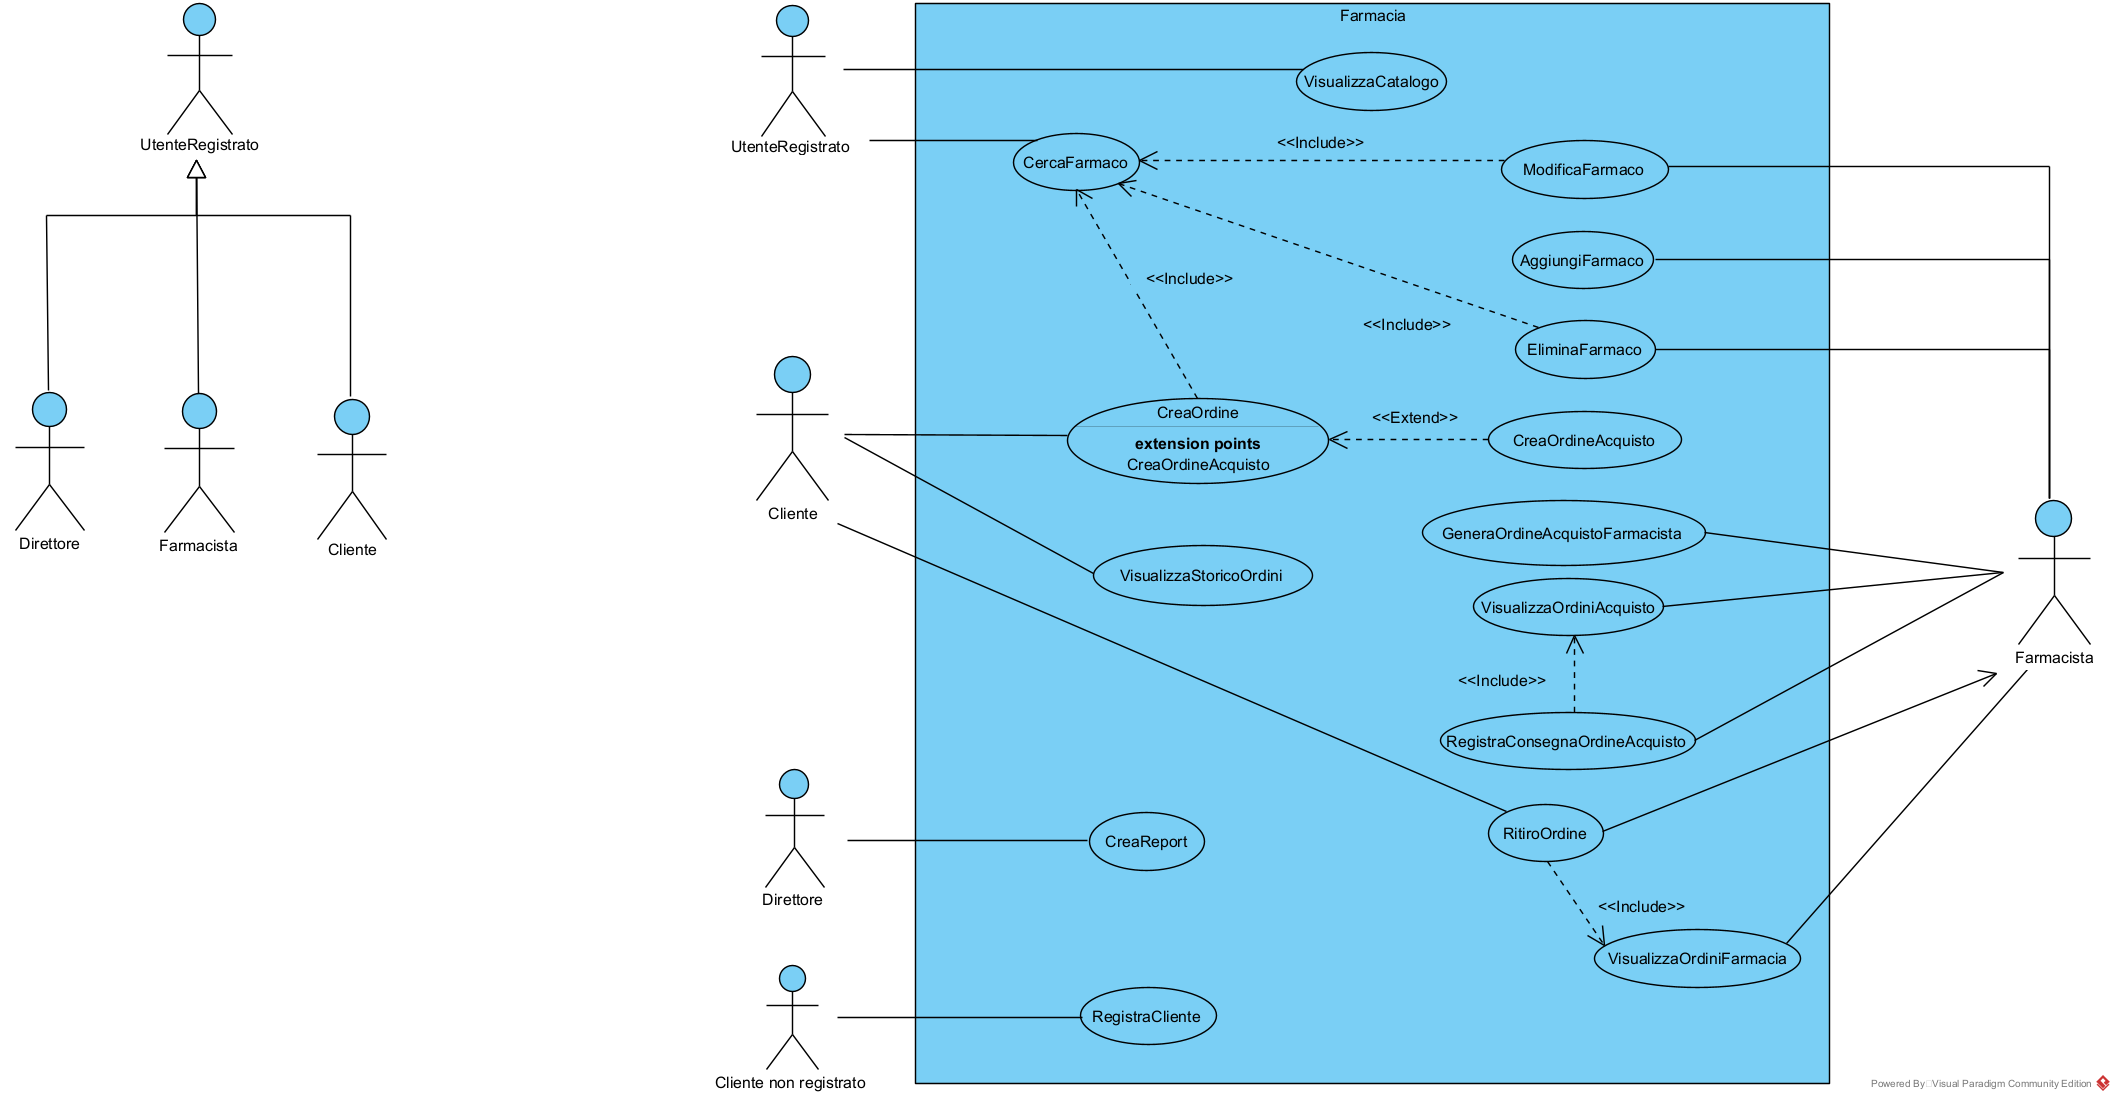
\includegraphics[width=\linewidth]{assets/UseCaseFarmacia.png}

\pagebreak

\section{Scenari}

\IncludeTable[!hbp]{chapters/usecases/RegistraCliente} % input
\IncludeTable[!hpt]{chapters/usecases/GeneraReport}
\IncludeTable[!hbp]{chapters/usecases/ModificaFarmaco}
\IncludeTable[!hbp]{chapters/usecases/AggiungiFarmaco}
\IncludeTable[!hbp]{chapters/usecases/EliminaFarmaco}
\IncludeTable[!hbp]{chapters/usecases/CercaFarmaco}
\IncludeTable[!hpt]{chapters/usecases/VisualizzaCatalogo}
\IncludeTable[!hpt]{chapters/usecases/VisualizzaOrdiniAcquisto}
\IncludeTable[!hpt]{chapters/usecases/RegistraConsegnaOrdineAcquisto}
\IncludeTable[!hpt]{chapters/usecases/VisualizzaOrdiniFarmacia}
\IncludeTable[!hpt]{chapters/usecases/VisualizzaStoricoOrdini}
\IncludeTable[!hpt]{chapters/usecases/RitiraOrdine}
\IncludeTable[!hpt]{chapters/usecases/GeneraOrdineAcquistoFarmacista}
\IncludeTable[!hpt]{chapters/usecases/CreaOrdine}
\IncludeTable[!hpt]{chapters/usecases/GeneraOrdineAcquisto}

\section{Diagramma delle Classi}
Di seguito riportiamo il diagramma delle classi di analisi.
\begin{figure}[!ht]
	\centering
	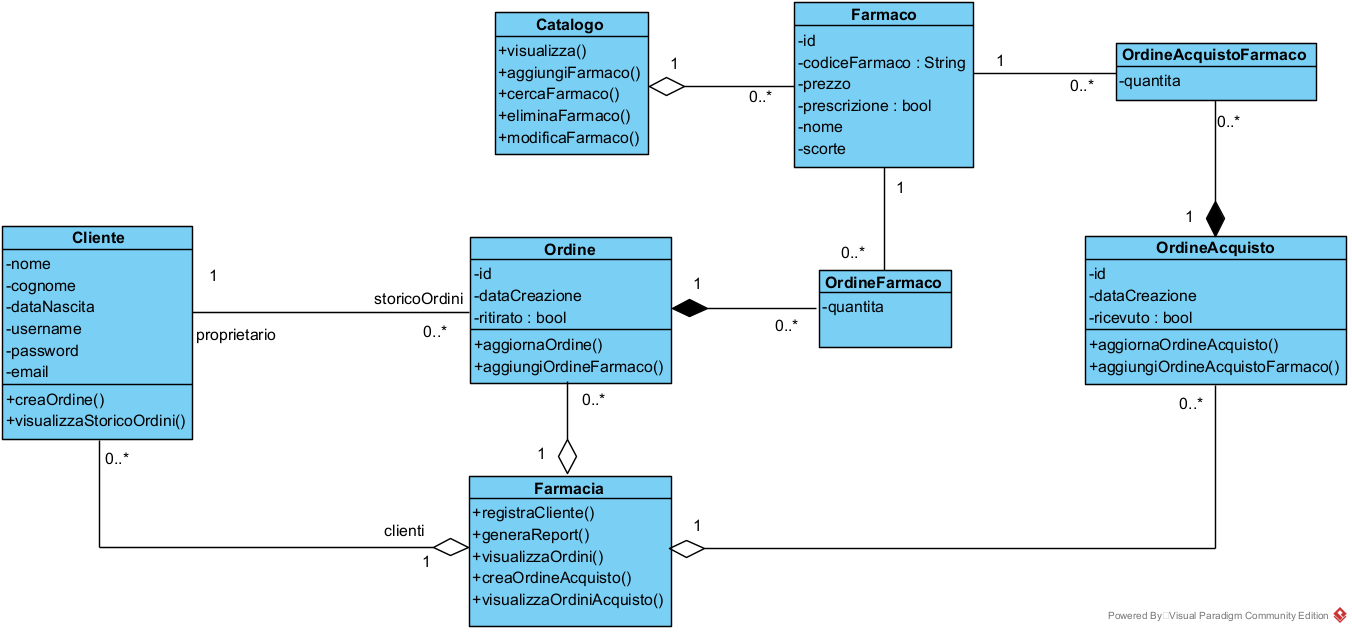
\includegraphics[width=\linewidth]{assets/ClassDiagramAnalisi.png}
	\caption{Diagramma delle classi di analisi}
\end{figure}

\section{Diagrammi di Sequenza}

\begin{figure}[!h]
	\centering
	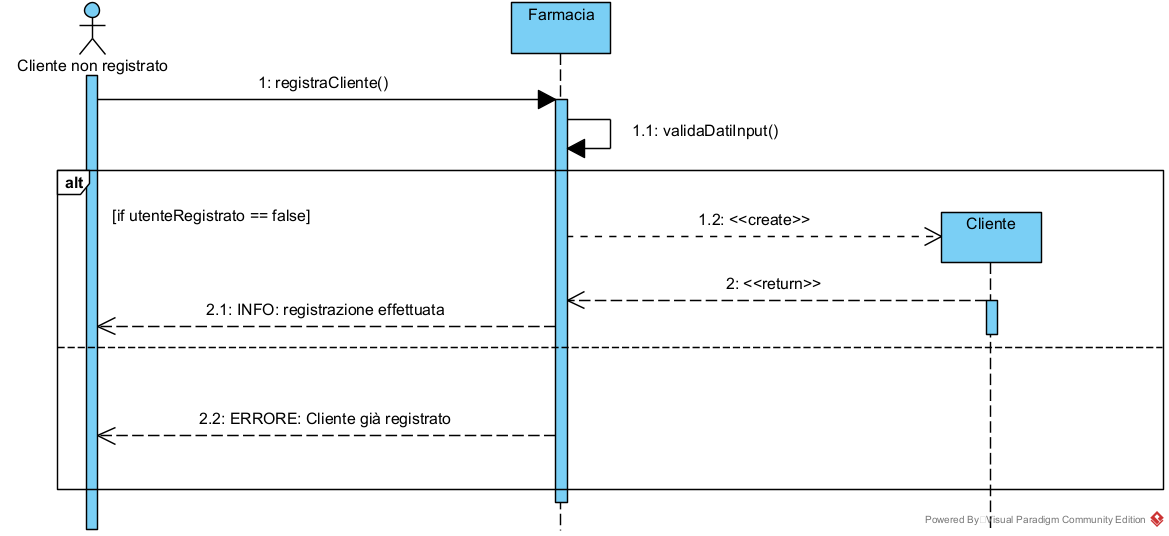
\includegraphics[width=\linewidth]{assets/sequence_analisi/RegistraCliente.png}
	\caption{Diagramma di sequenza di analisi di RegistraCliente}
\end{figure}

\vfill
\pagebreak

\begin{figure}[!hbp]
	\centering
	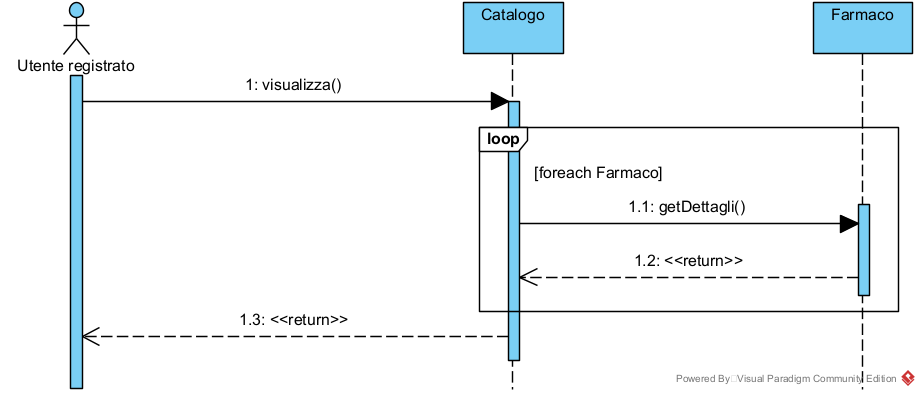
\includegraphics[width=0.8\linewidth]{assets/sequence_analisi/VisualizzaCatalogo.png}
	\caption{Diagramma di sequenza di analisi di VisualizzaCatalogo}
\end{figure}

\begin{figure}[!hbp]
	\centering
	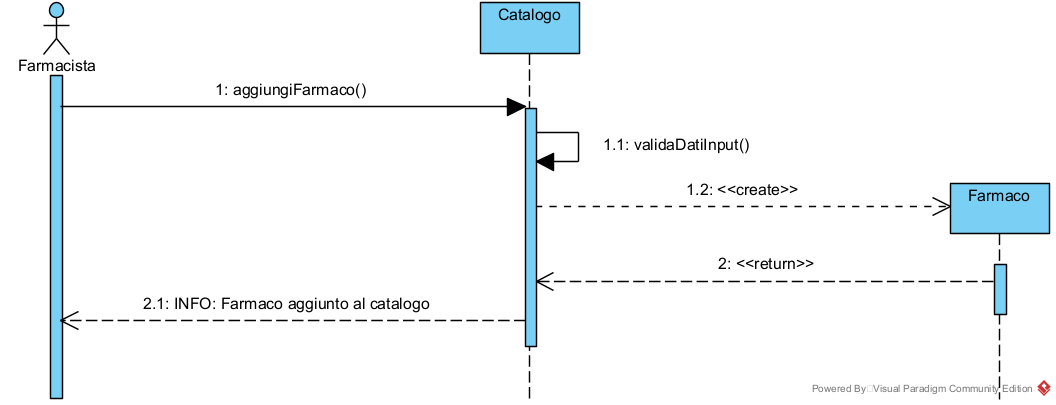
\includegraphics[width=\linewidth]{assets/sequence_analisi/AggiungiFarmaco.png}
	\caption{Diagramma di sequenza di analisi di AggiungiFarmaco}
\end{figure}

\begin{figure}[!hbp]
	\centering
	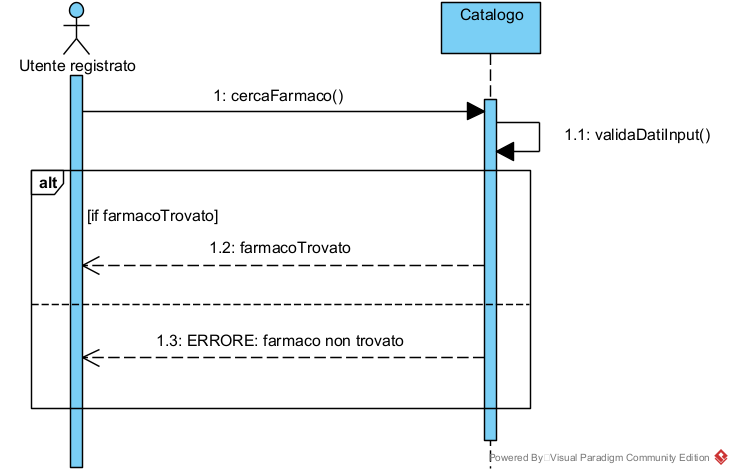
\includegraphics[width=0.7\linewidth]{assets/sequence_analisi/CercaFarmaco.png}
	\caption{Diagramma di sequenza di analisi di CercaFarmaco}
\end{figure}

\begin{figure}[!hbp]
	\centering
	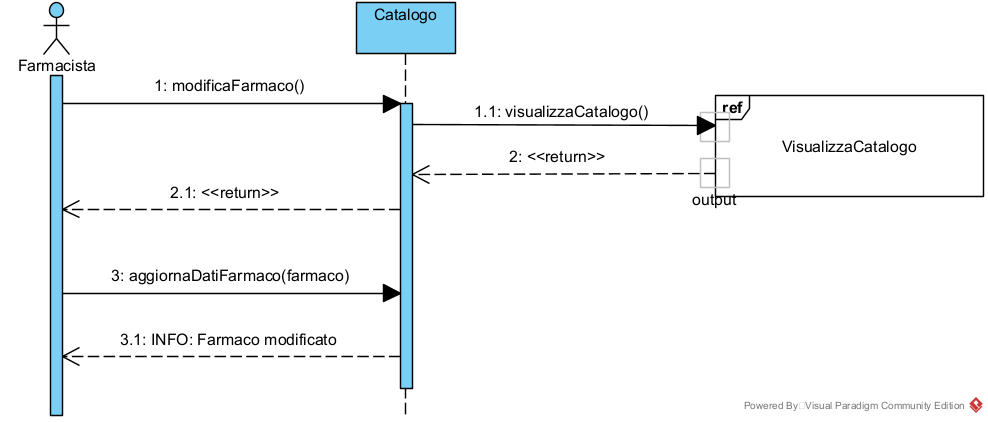
\includegraphics[width=0.8\linewidth]{assets/sequence_analisi/ModificaFarmaco.png}
	\caption{Diagramma di sequenza di analisi di ModificaFarmaco}
\end{figure}

\begin{figure}[!hbp]
	\centering
	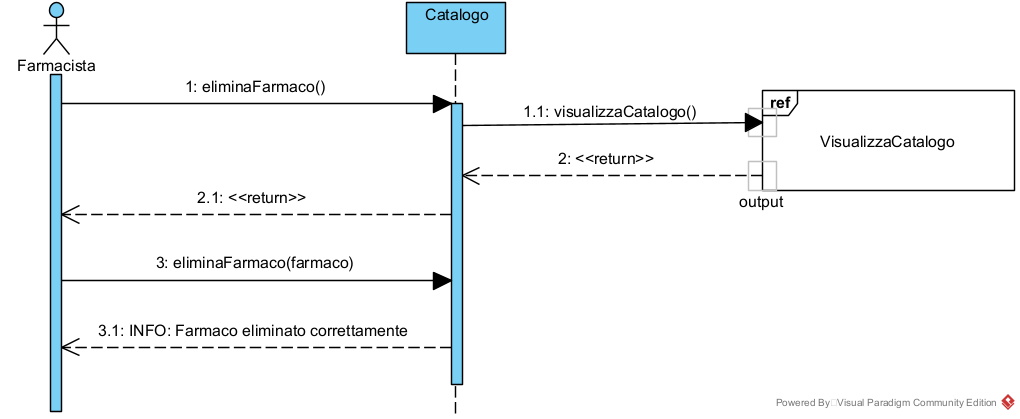
\includegraphics[width=0.8\linewidth]{assets/sequence_analisi/EliminaFarmaco.png}
	\caption{Diagramma di sequenza di analisi di EliminaFarmaco}
\end{figure}

\begin{figure}[!hbp]
	\centering
	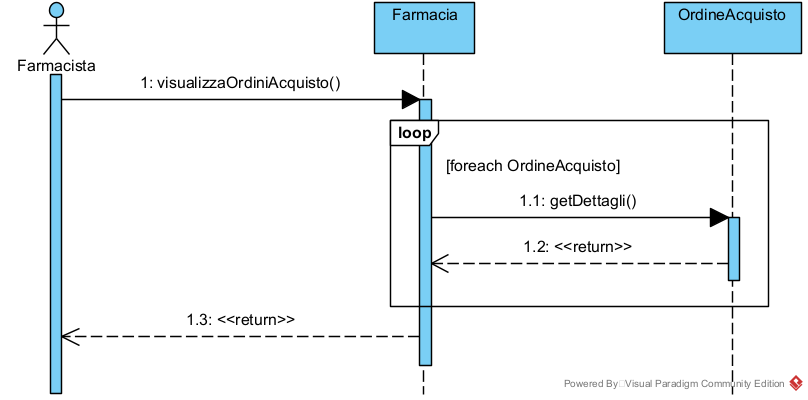
\includegraphics[width=0.8\linewidth]{assets/sequence_analisi/VisualizzaOrdiniAcquisto.png}
	\caption{Diagramma di sequenza di analisi di VisualizzaOrdiniAcquisto}
\end{figure}

\begin{figure}[!hbp]
	\centering
	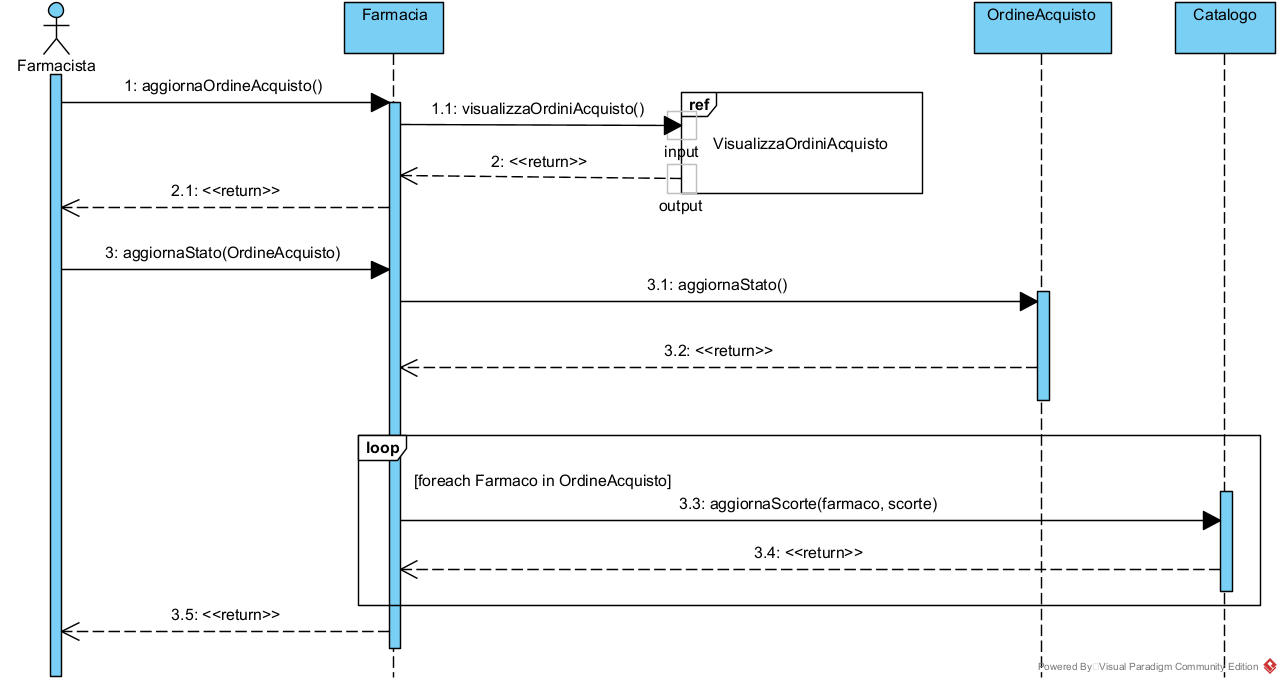
\includegraphics[width=\linewidth]{assets/sequence_analisi/AggiornaOrdineAcquisto.png}
	\caption{Diagramma di sequenza di analisi di AggiornaOrdineAcquisto (RegistraConsegnaOrdineAcquisto)}
\end{figure}

\begin{figure}[!hbp]
	\centering
	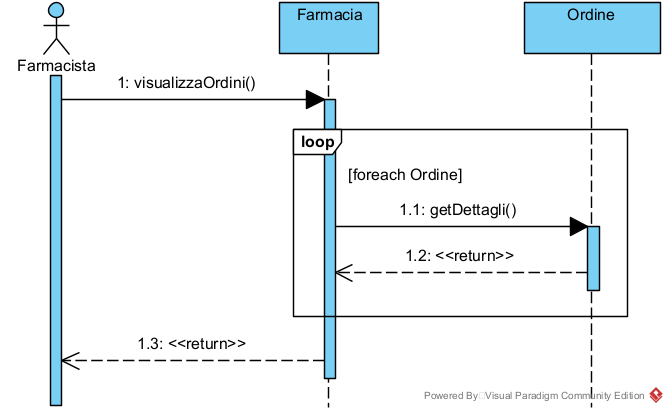
\includegraphics[width=0.9\linewidth]{assets/sequence_analisi/VisualizzaOrdiniFarmacia.png}
	\caption{Diagramma di sequenza di analisi di VisualizzaOrdiniFarmacia}
\end{figure}

\begin{figure}[!hbp]
	\centering
	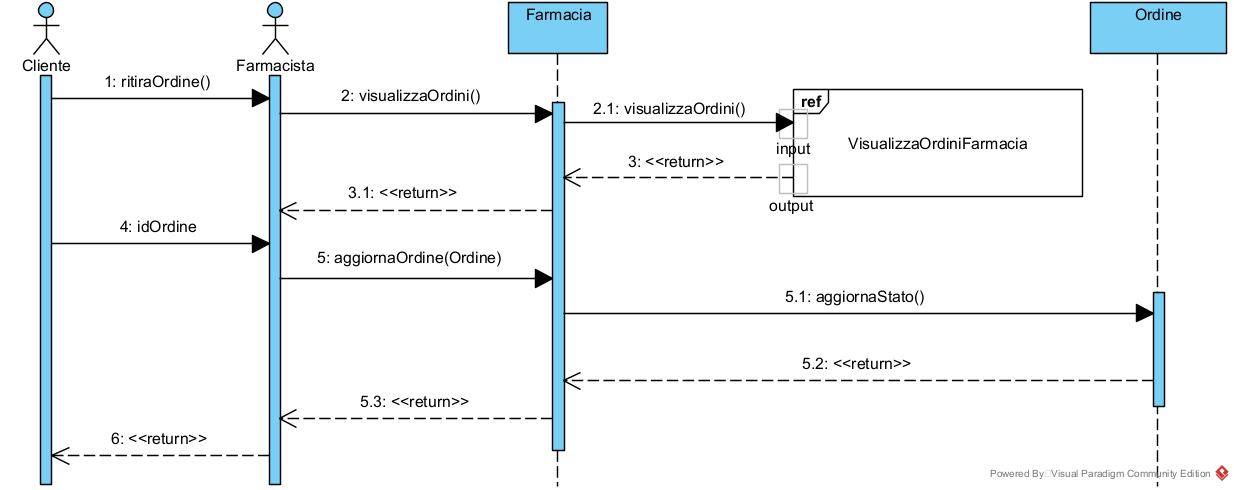
\includegraphics[width=\linewidth]{assets/sequence_analisi/RitiraOrdine.png}
	\caption{Diagramma di sequenza di analisi di RitiraOrdine}
\end{figure}

\begin{figure}[!hbp]
	\centering
	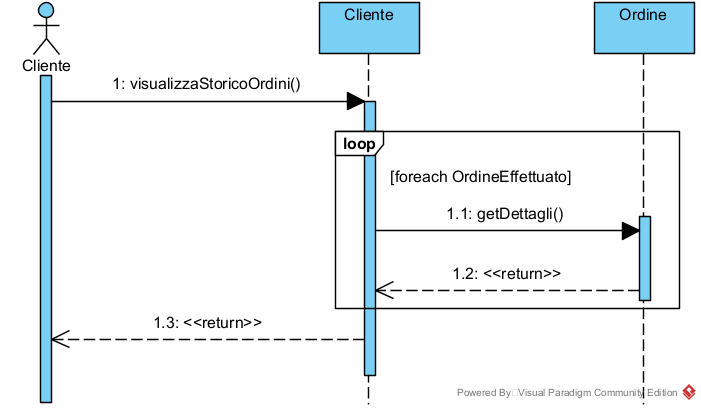
\includegraphics[width=0.8\linewidth]{assets/sequence_analisi/VisualizzaStoricoOrdini.png}
	\caption{Diagramma di sequenza di analisi di VisualizzaStoricoOrdini}
\end{figure}

\begin{figure}[!hbp]
	\centering
	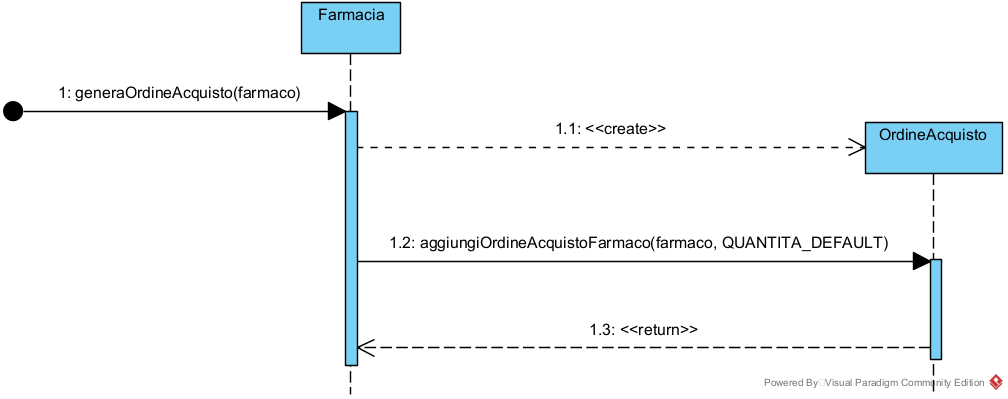
\includegraphics[width=0.9\linewidth]{assets/sequence_analisi/GeneraOrdineAcquisto.png}
	\caption{Diagramma di sequenza di analisi di GeneraOrdineAcquisto}
\end{figure}

\begin{figure}[!hbp]
	\centering
	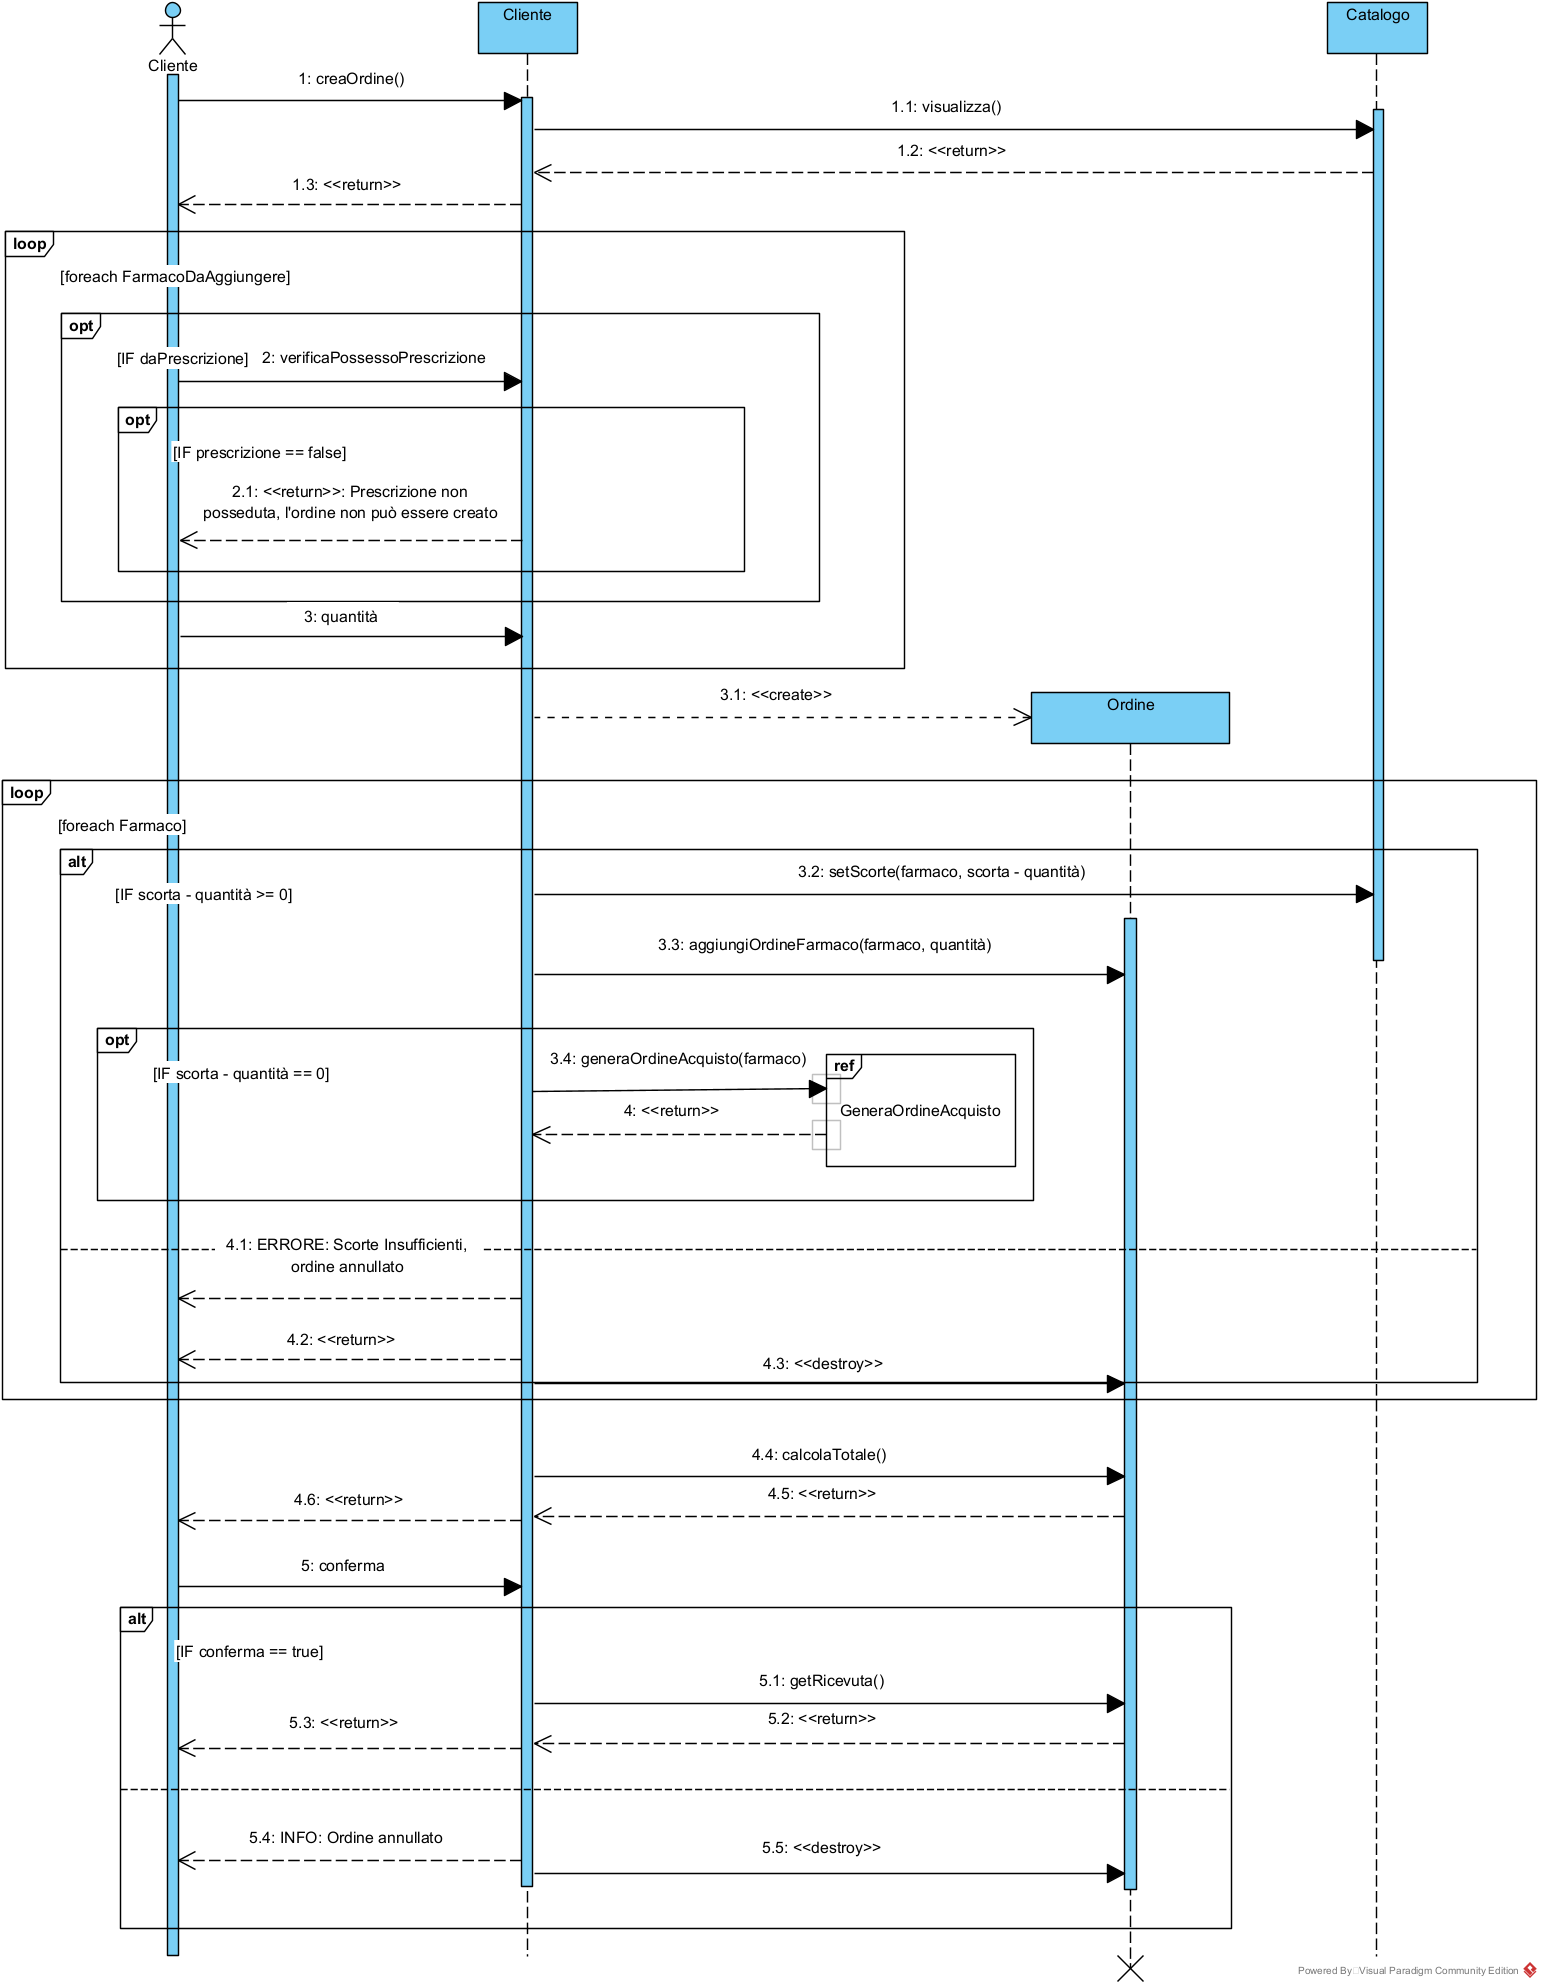
\includegraphics[width=\linewidth]{assets/sequence_analisi/CreaOrdine.png}
	\caption{Diagramma di sequenza di analisi di CreaOrdine}
\end{figure}

\begin{figure}[!hbp]
	\centering
	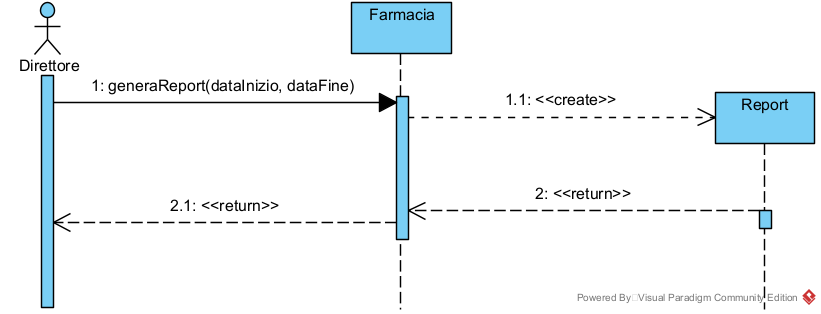
\includegraphics[width=0.9\linewidth]{assets/sequence_analisi/GeneraReport.png}
	\caption{Diagramma di sequenza di analisi di GeneraReport}
\end{figure}

\begin{figure}[!hbp]
	\centering
	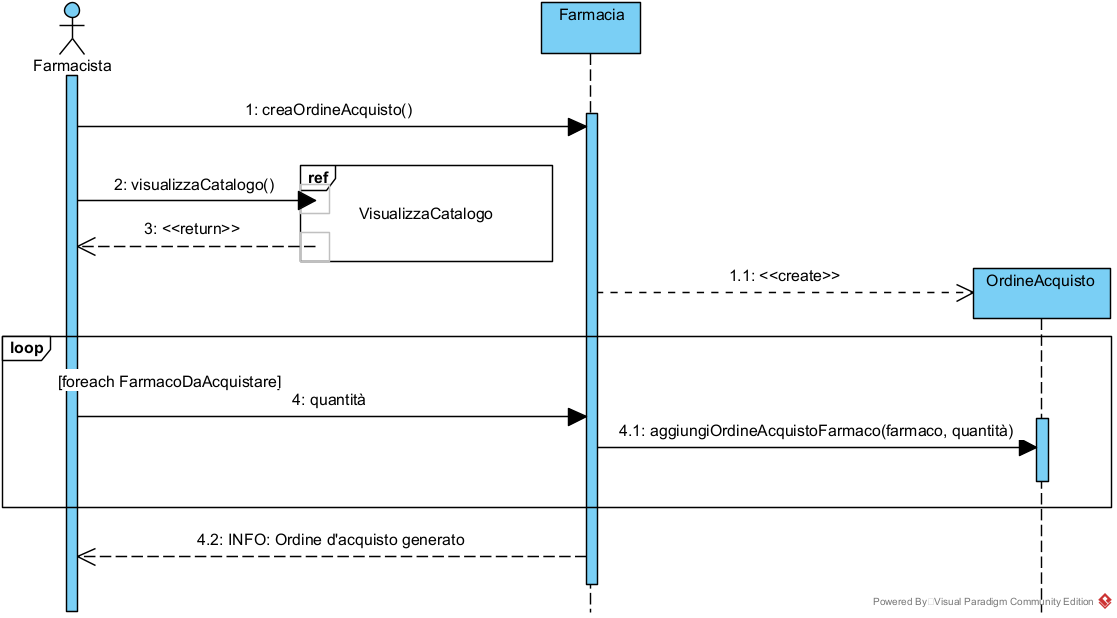
\includegraphics[width=\linewidth]{assets/sequence_analisi/GeneraOrdineAcquistoFarmacista.png}
	\caption{Diagramma di sequenza di analisi di GeneraOrdineAcquistoFarmacista}
\end{figure}

\section{Verifica Completezza dei Requisiti}

\begin{itemize}
	\item \Req{rf}{01}, \Req{rf}{06} Modellati in UCD da VisualizzaCatalogo con l'attore UtenteRegistrato
	\item \Req{rf}{02} Modellato in UCD da AggiungiFarmaco con l'attore primario Farmacista
	\item \Req{rf}{03} Modellato in UCD da ModificaFarmaco con l'attore primario Farmacista
	\item \Req{rf}{04} Modellato in UCD da EliminaFarmaco con l'attore primario Farmacista
	\item \Req{rf}{05} Modellato in UCD da RegistraCliente con l'attore primario Cliente non Registrato
	\item \Req{rf}{07}, \Req{rf}{08}, \Req{rf}{09}, \Req{rf}{10}, \Req{rf}{17} Modellati in UCD da CreaOrdine con l'attore primario Cliente
	\item \Req{rf}{11} Modellato in UCD da VisualizzaOrdiniAcquisto con l'attore primario Farmacista
	\item \Req{rf}{12} Modellato in UCD da RegistraConsegnaOrdineAcquisto con l'attore primario Farmacista
	\item \Req{rf}{13} Modellato in UCD da GeneraReport con l'attore primario Direttore
	\item \Req{rf}{14} Modellato in UCD da VisualizzaOrdiniFarmacia con l'attore primario Farmacista
	\item \Req{rf}{15} Modellato in UCD da RitiraOrdine con l'attore primario Cliente e attore secondario Farmacista
	\item \Req{rf}{16} Modellato in UCD da VisualizzaStoricoOrdini con l'attore primario Cliente
	\item \Req{rf}{18} Modellato in UCD da CercaFarmaco con l'attore primario UtenteRegistrato
	\item \Req{rf}{19} Modellato in UCD da GeneraOrdineAcquistoFarmacista con l'attore primario Farmacista
	\item \Req{rd}{01}, \Req{rd}{02} Modellato nel CD dalla classe Farmaco
	\item \Req{rd}{03} Modellato nel CD dalla classe Cliente
	\item \Req{rd}{04} Modellato nel CD dalla classe Report
\end{itemize}

\begin{table}[!hbp]
	\centering
	\begin{tblr}{
		colspec = lllll,
		hlines = {1pt}, colsep = 12pt
		}
		UCD = Use Case Diagram & CD = Class Diagram & SD = Sequence Diagram \\
	\end{tblr}
\end{table}
